\documentclass[12pt,fleqn,a4paper]{article}

\usepackage{latexsym}
\usepackage{url}
\usepackage{xspace}
\usepackage{epsfig}
\usepackage{psfrag}
\usepackage{a4wide}
\usepackage{marvosym}
\usepackage{amsmath,amsfonts,amssymb,amsthm,latexsym}
\usepackage{graphics,graphicx,color,subfigure}
\usepackage{fancyhdr}
\usepackage[english]{babel}
\usepackage[latin1]{inputenc}

\textheight 680pt
\textwidth 460pt
\topmargin -40pt
\oddsidemargin 5pt
\evensidemargin 5pt
\parindent 0pt

\pagestyle{fancyplain} \setlength{\headheight}{16pt}
\renewcommand{\sectionmark}[1]{\markright{\thesection\ #1}}
\lhead[\fancyplain{}{\thepage}]
    {\fancyplain{}{\rightmark}}
\rhead[\fancyplain{}{\leftmark}]
    {\fancyplain{}{\thepage}}
\cfoot{}
\renewcommand{\thesection}{\arabic{section}}
\renewcommand{\thesubsection}{\arabic{section}.\arabic{subsection}}


\begin{document}
\begin{titlepage}%Institution
\vspace{2cm}
\centerline{
\large{Department of Computer Sciences}}
\vspace{0.2cm}
\centerline{\large{University of Salzburg}}%Title with one or two Lines(More if wanted)
%\hline
\vspace{2cm}

\centerline{\large{PS Natural Computation}}
\centerline{SS 15/16}
\vspace{1cm}

\centerline{\Large{\bf{Evolution of a Poker Player Using Genetic Programming}} }%Type of the Document
\vspace{1cm}

\vspace{0.4cm}%Date
\centerline{\today}
\vspace{4.5cm}%Authors

%\hline
\vspace{0.2cm}
Project Members:\\
\centerline{Thomas Samy Dafir, 1331483, tdafir@cosy.sbg.ac.at}\\
\centerline{Laurentiu Vlad, 1423336, lvlad@cosy.sbg.ac.at}\\
\centerline{Dominik Baumgartner, 0920177, dbaumgart@cosy.sbg.ac.at}\\
\centerline{Sebastian Strumegger, 1420277, sstrumegg@cosy.sbg.ac.at}\\
\vspace {1cm}\\

Academic Supervisor: \\
\centerline{Helmut MAYER}
\centerline{helmut@cosy.sbg.ac.at}
\vspace{1.5cm}\\
Correspondence to: \\
\centerline{Universit\"{a}t Salzburg} \\
\centerline{Fachbereich Computerwissenschaften} \\
\centerline{Jakob--Haringer--Stra\ss e 2} \\
\centerline{A--5020 Salzburg} \\
\centerline{Austria}
\clearpage
\end{titlepage}

%Table of Content
% \setcounter{page}{1}
% \pagenumbering{Roman} %I,II,III... in the TOC
% \tableofcontents

\clearpage
\pagestyle{headings}
\pagenumbering{arabic}  %Better if TOC is variable (more than one page)
\setcounter{page}{1}
\pagenumbering{arabic}  %Better if TOC is variable (more than one page)
\setcounter{page}{1}

\abstract{
The goal of this project is to evolve a GP poker player by means of genetic programming techniques.
The GP Players evolve over generations through selection, mutation and cross mutation of their chromosome tree. \\
A good computer player has to emerge after a sufficient amount of generations have been played in a "heads up" texas-hold-em no limit poker game.
Good players are determined by their fitness value which is determined through assessing a player's success after each poker round. \\
The focus of our work lies in the chromosome tree.
Although the current API provides some basics functions for that tree, it is likely that they are not sufficient for the evolution of a good player.
The second focus lies on the poker game itself.
We have to determine what kind and how much information a player needs in order to evolve properly without interfering with its evolution.
This means, that we don't want to "tell" the player what the next best action is, but rather let evolution decide.
Additionally we will do some fine-tuning of evolutionary-parameters like population size or number of generations to achieve the best possible result.
}

\newpage

\section{Genetic Programming}
As mentioned, a GP Player is represented by a so-called chromosome tree. Or more exactly, the poker player's strategy is represented by this tree.\\
This means, that each player's tree has a root node and more or less child nodes, where nodes with children are called functions and leave nodes are called terminals.\\
From the very beginning there is a fixed set of functions and terminals available.
At first, a population of GP Players with random nodes are created which play a predetermined number of games.
In each generation there is a chance for every player that it's tree is changed by mutation or crossover.

\subsection{Chromosome Tree}
\subsubsection{Functions}
Functions play the most important role in a GP Player's strategy, since functions are the decision-makers.\\
They can have one or more child nodes and always are of a specific return type. Further they need to have a parent node (except the root function).
Child nodes can either be terminals or functions, where it is also very important that the child nodes return the very type, that the function expects.\\
As an example we could define a lower-than function that expects floating point values from both children and returns a boolean value to it's parent node.

\subsubsection{Terminals}
Terminals are the leave nodes in a player's tree. They cannot have child nodes but return a certain type themselves.\\
This does not necessarily mean that a terminal's value has to be static. They can have dynamic values like "pot size" or "higher hand card". 

\subsubsection{Root}
The root node it a special function, since it does not have any parent nodes.\\
For a proper evaluation of the player's tree it needs to be rooted, so we can start making further decisions at one point.
For GPoker we need to have a root node that allways returns a poker move which is returned to the game.\\
~\\
A GPlayer, for example, uses the root node "IfMove" which has three children:\\
The very left child is the if-branch, that needs to return a boolean type.\\
The middle child is the then-branch and returns a move.\\
And at last, the right child represents the else-branch, which also returns a move.\\

\newpage

\subsubsection{Example}
\begin{center}
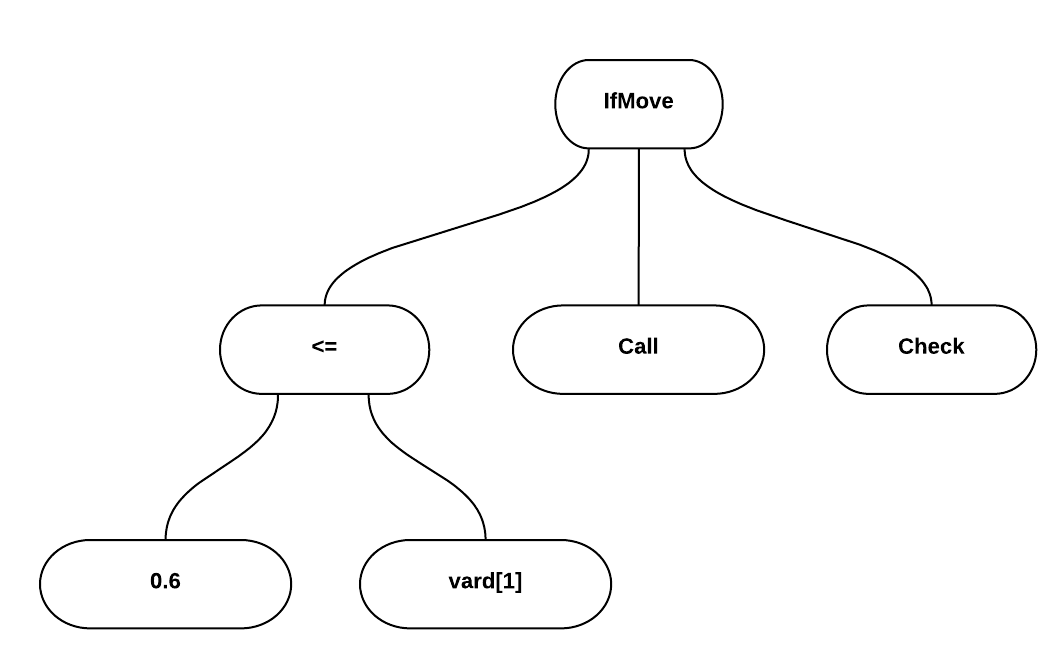
\includegraphics[width=0.8\textwidth]{tree1.png}
\end{center}
This very simple tree represents the following strategy:
~\\
If 0.6 (Two to Ace normalized in 0 to 1) is less than or equal to the player's lower hand card, make a call.\\
Else, check the game. Note that checking can also mean folding, in case there has been a raise.

\subsection{Evolution}
There are two fundamentally different ways for evolution to change a tree, namely crossover and mutation.

\subsubsection{Crossover}
Crossover takes two individual players and swaps subtrees in a random point.
Of course both subtrees need to have the same return type.
This method is more common, since good players that were not sorted out by evolution usually have good subtrees.
So the the well-playing trees are not completely destroyed by the process of evolution, but there is much room for new combinations.

\begin{center}
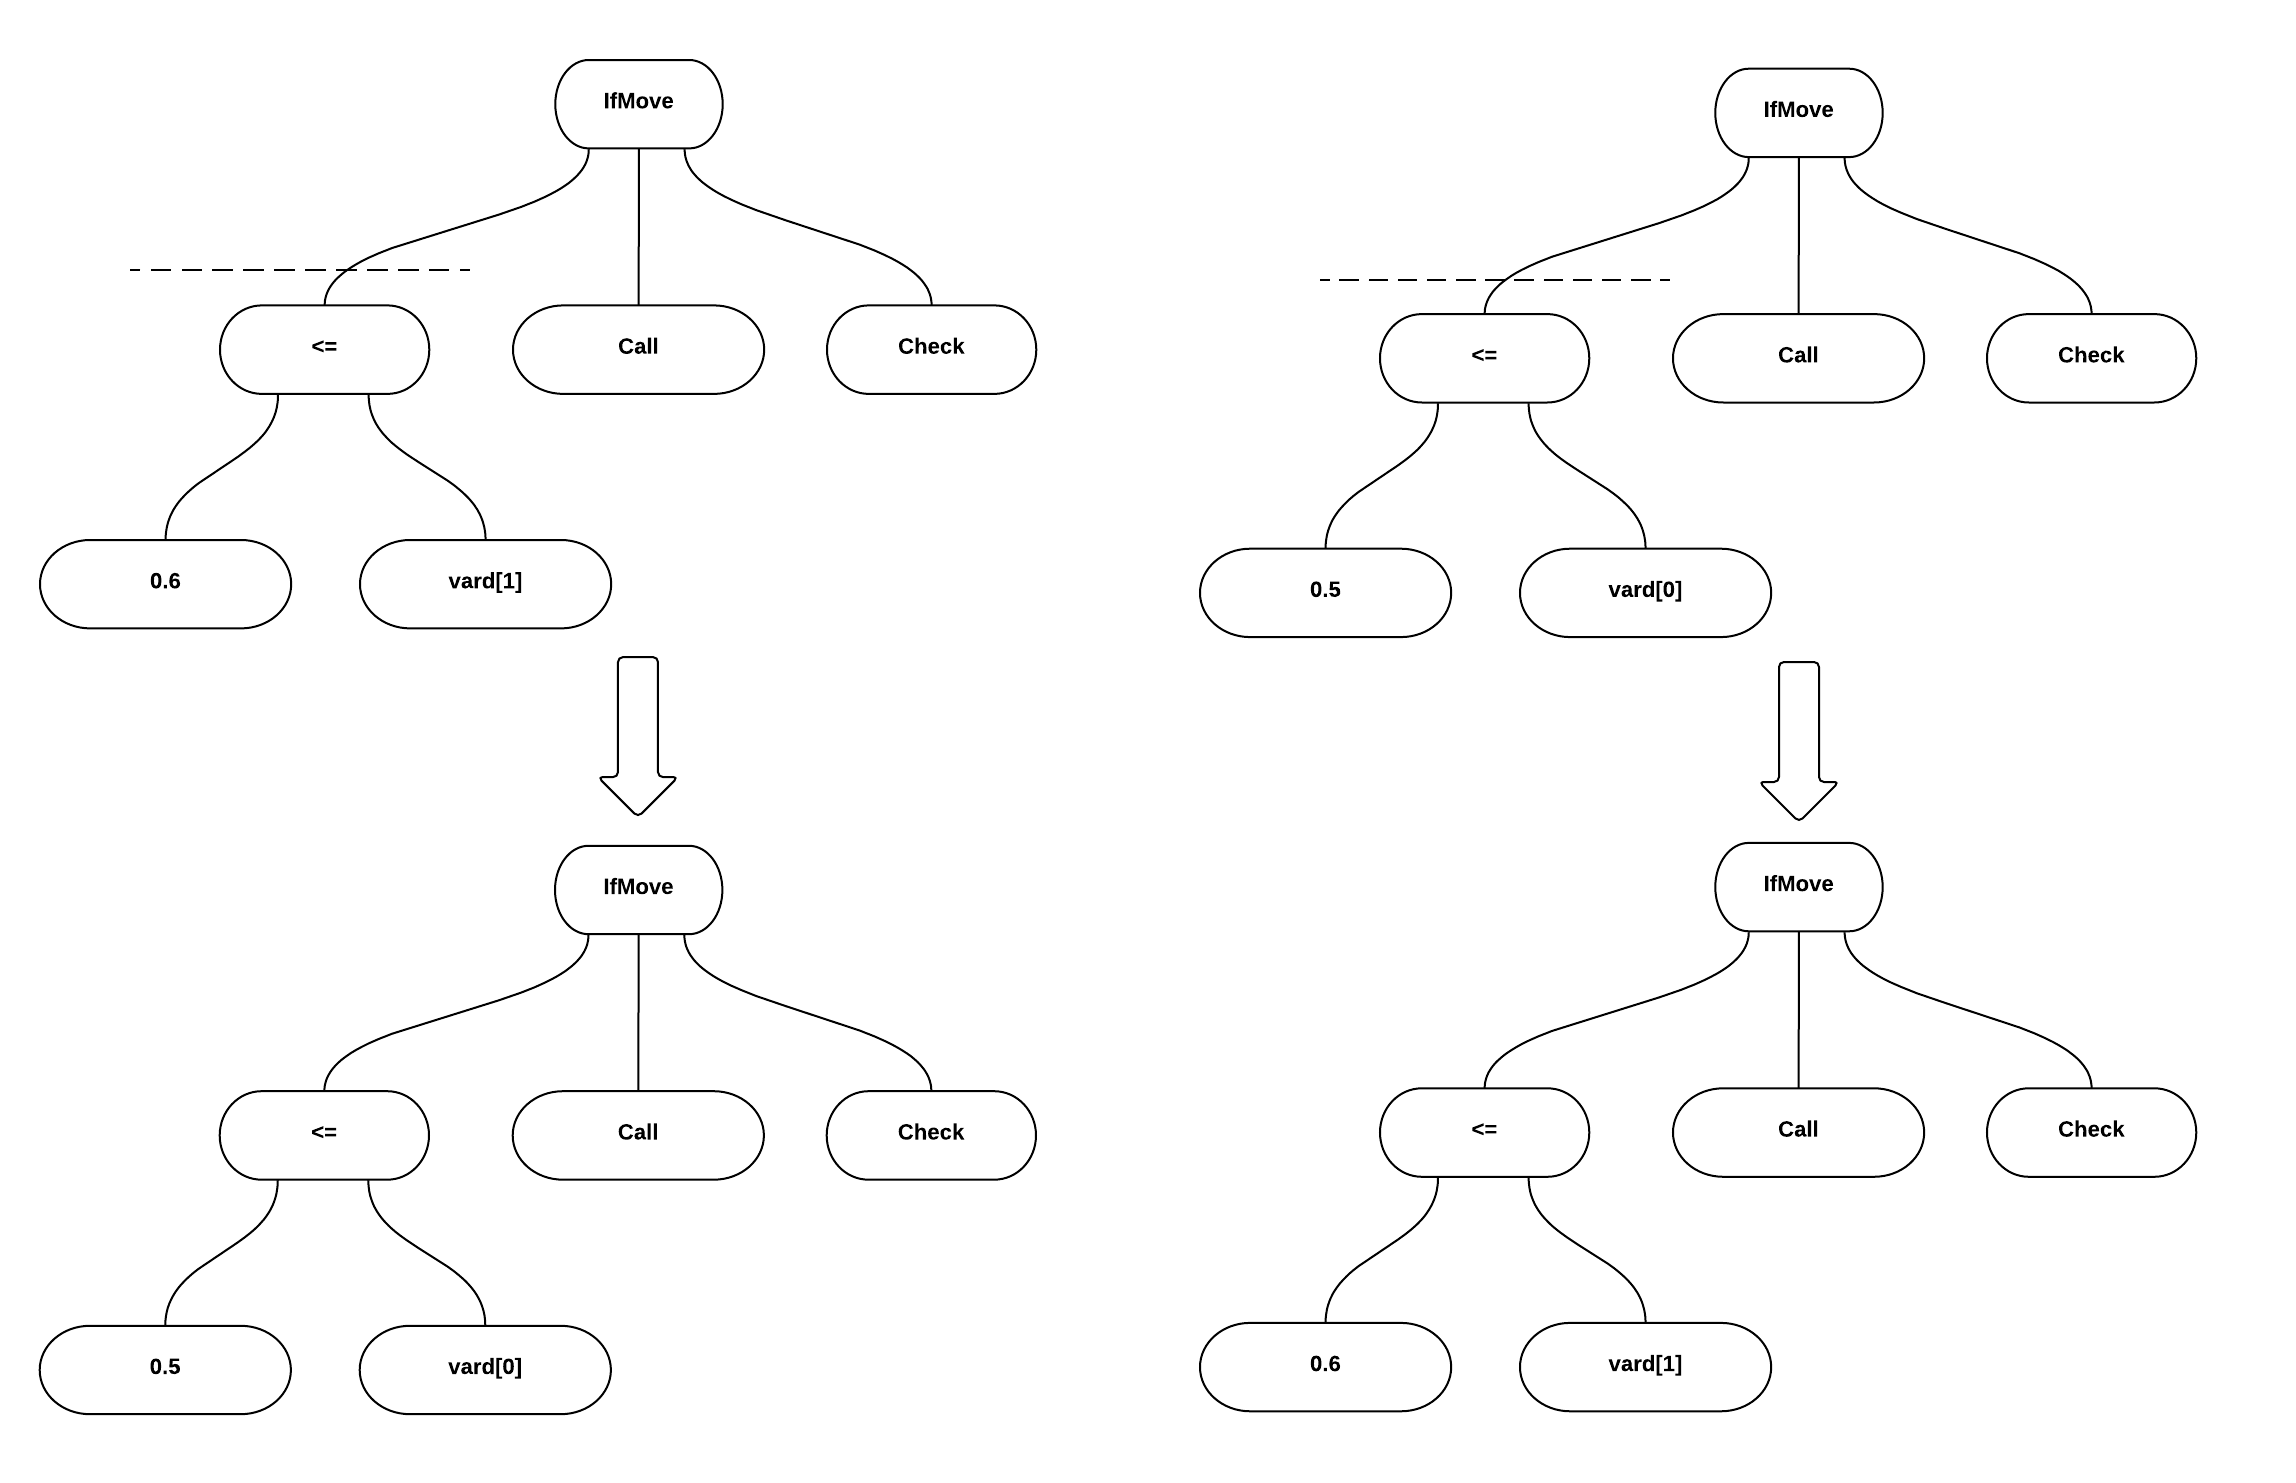
\includegraphics[width=1.0\textwidth]{tree_crossover.png}
\end{center}

\subsubsection{Mutation}
In contrast to Crossover, mutation does not even need two individual trees for change.
Either a single node is chosen randomly and changed to some other random node that returns the same type.
Or even a randomly chosen subtree can be changed.
Mutation has to be used carefully, since random changes can change a very good player to be useless.

\begin{center}
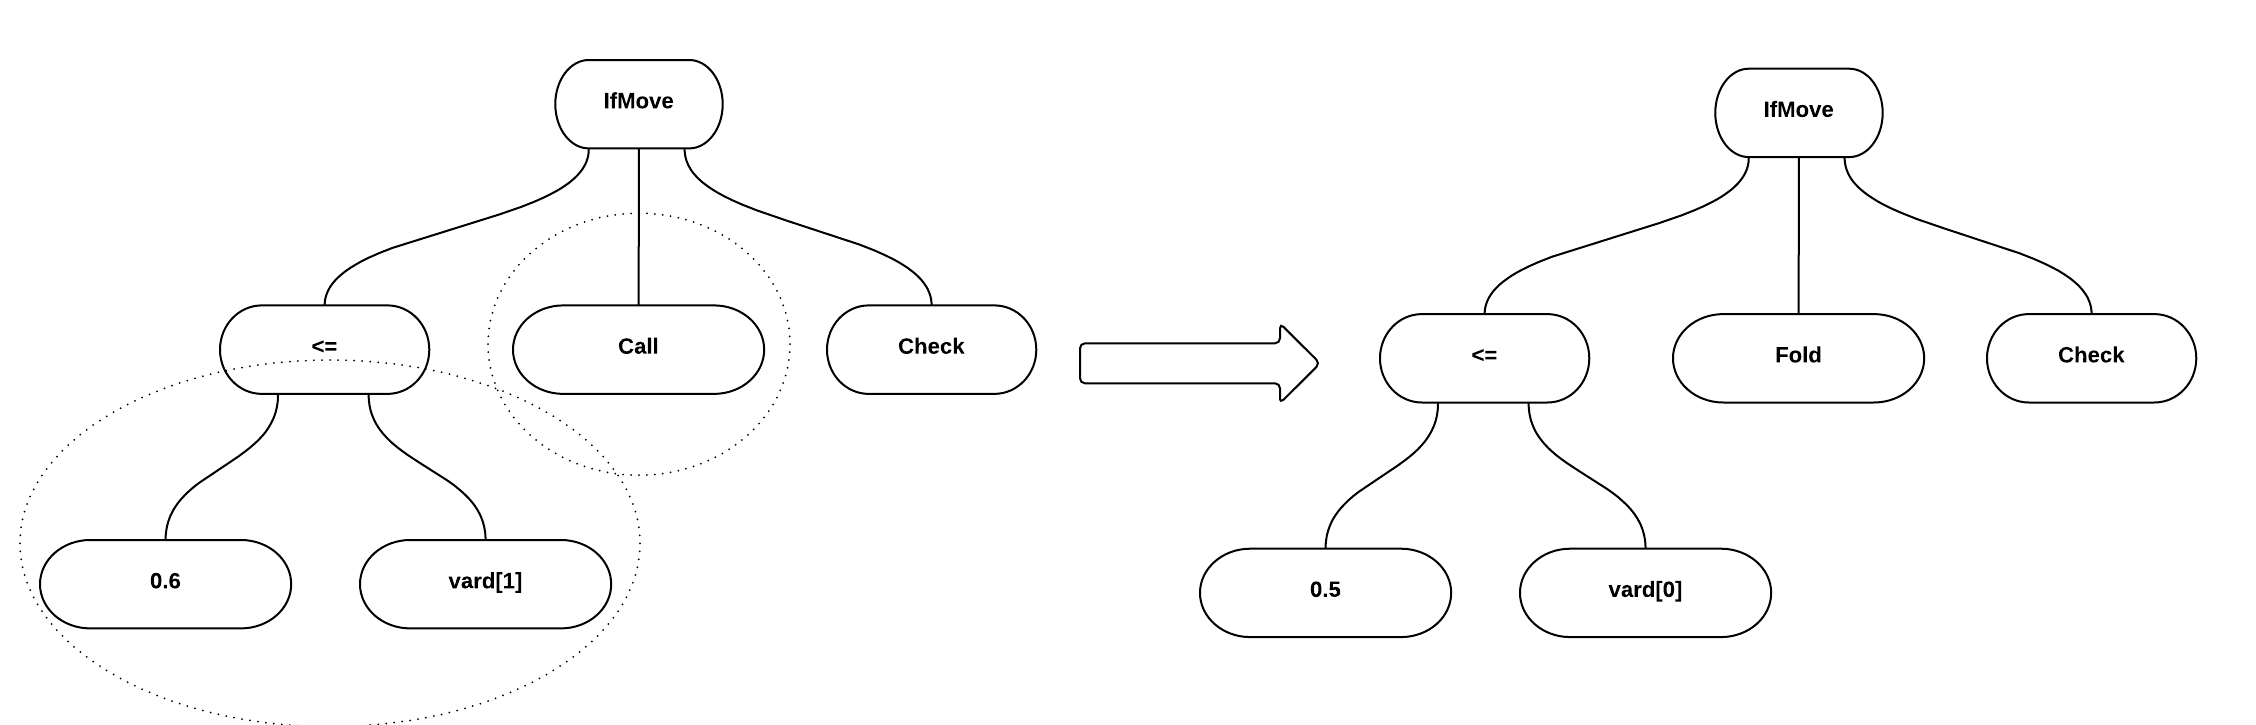
\includegraphics[width=1.0\textwidth]{tree_mutation.png}
\end{center}

\newpage

% links go here, NOT in references

\section{Links}

\begin{itemize}
\item Project Page: \url{https://student.cosy.sbg.ac.at/~tdafir/nc/}
\item PS Page:
\url{http://www.cosy.sbg.ac.at/~helmut/Teaching/NaturalComputation/proseminar.html}

\end{itemize}

\nocite{*}
\bibliographystyle{ieeetr}
\bibliography{report_refs.bib}		% .bib files here

\end{document}
